\documentclass{article}

% Language setting
% Replace `english' with e.g. `spanish' to change the document language
\usepackage[english]{babel}

% Set page size and margins
% Replace `letterpaper' with `a4paper' for UK/EU standard size
\usepackage[a4paper,top=2cm,bottom=2cm,left=3cm,right=3cm,marginparwidth=1.75cm]{geometry}

% Useful packages
\usepackage{amsmath}
\usepackage{graphicx}
\usepackage[colorlinks=true, allcolors=blue]{hyperref}
\usepackage{xcolor}
\usepackage{listings}
\usepackage{dirtytalk}

\colorlet{mygray}{black!30}
\colorlet{mygreen}{green!60!blue}
\colorlet{mymauve}{red!60!blue}

\lstset{
  backgroundcolor=\color{gray!10},  
  basicstyle=\ttfamily,
  columns=fullflexible,
  breakatwhitespace=false,      
  breaklines=true,                
  captionpos=b,                    
  commentstyle=\color{mygreen}, 
  extendedchars=true,              
  frame=single,                   
  keepspaces=true,             
  keywordstyle=\color{blue},      
  language=c++,                 
  numbers=none,                
  numbersep=5pt,                   
  numberstyle=\tiny\color{blue}, 
  rulecolor=\color{mygray},        
  showspaces=false,               
  showtabs=false,                 
  stepnumber=5,                  
  stringstyle=\color{mymauve},    
  tabsize=3,                                     
  title=\lstname 
}


\lstnewenvironment{code}[2][]{%
  \lstset{%
    numbers = left,
    title   = #2,
    #1,
  }%
}{}

\title{Homework 2 \\ \big{Mechatronics II}}
\author{Steinarr Hrafn Höskuldsson}

\newcommand{\mycomment}[1]{}
\usepackage{fancyhdr}
\fancypagestyle{firststyle}
{
   \fancyhf{}
   \fancyhead[L]{Mechatronics 2}
   
   \renewcommand{\headrulewidth}{0pt} % removes horizontal header line
}
\begin{document}

\mycomment{

\begin{figure}[h]
    \centering
    \includegraphics[width=0.75\textwidth]{LAB3/Basic1.png}
    \caption{"Switch test" Breadboard set up}
    \label{fig:Switch_test}
\end{figure}

\lstinputlisting[caption=Defining 'ColorMatch' state, label={lst:colormatch}, language=Python, firstline=44, lastline=52]{LAB3/Basic.py}

} % end of comment

\pagestyle{firststyle}
{\let\newpage\relax\maketitle}

\section*{Problems}

\subsection*{ What numbers (e.g. range) can a byte (8 bits) and an integer (16 bits) describe?}
A byte, consisting of 8 bits can describe $2^8 = 256$ unique numbers. If the byte is signed the range is $\{-128 .. 127\}$ but if the byte is unsigned the range is $\{0 .. 255\}$. Similarly a 16 bit integer can describe $2^{16}$ different numbers. If the integer is signed the range is $\{-32,768 .. 32,767\}$ but an unsigned integer covers the range $\{0 .. 65535\}$
\subsection*{ Write the bit pattern (e.g. hex) for the integer $1962_D$ (D for Decimal)}
$1962_D = 1024 + 512 + 256 + 128 + 32 + 8 + 2 = 2^{10} + 2^9 + 2^8 + 2^7 + 2^5 + 2^3 + 2^1 = 0000\;0111\;1010\;1010_B$

\subsection*{ Write the bit pattern (e.g. hex) for the byte  -13D}
First find the bit pattern for $13_D = 0000\;1101_B$ then use 2's compliment to get:\\
$-13_D = 1111\;0010_B + 1_B = 1111\;0011_B$
\subsection*{ Write the bit pattern (e.g. hex) for the single precision number 1,0D}
The sign bit is 0, the exponent bits are $E=127_D = 0111\; 1111_B$ and the mantissa is 0 giving: $1.0_D = 0011\;1111\; 1000\; 0000\; 0000\; 0000\; 0000\; 0000_B = 3f80\;0000_H$
\subsection*{ And toghether bitwise the bitpatterns 0x55 and 0xAA}
$55_H \& AA_H = 0101\;0101_B \& 1010\; 1010_B = 0000\;0000 = 00_H$
\subsection*{ OR together the bitpatterns 0x55 and 0xAA}
$55_H\;\|\; AA_H = 0101\;0101_B \;\|\; 1010\; 1010_B = 1111\;1111_B = FF_H$
\subsection*{ Add together 0x55 and 0xAA}
in hexadecimal notation:
$55 + AA = 10*(A+5) + (A+5) = 10*F + F = FF$
\subsection*{ Subtract 0x55 from 0xAA}
In hexadecimal notation:
$AA - 55 = 10*(A-5) + (A-5) = 10*5 + 5 = 55$
\subsection*{ Write the bit pattern for ASCII symbol „A“}
From the ASCII table it can be read that „A“ has the hexadecimal code  $41_H$, thus has the bit pattern $0100\;0001_B$
\subsection*{ Show how do we define an signed 8-bit integer in C (not using any library)?}
On most systeSms a char is signed but not always so to make sure we should explicitly define it as signed:
\verb!signed char a;!
\subsection*{ Explain the AVR assembler command BREQ}
\verb!BREQ! stand for \textbf{Branch if Equal} it is a conditional branch. It compares two values and if they are equal it sends the program execution to a certain location, else it does nothing.

\subsection*{ Make a block diagram of your project}

\begin{figure}[h]
    \centering
    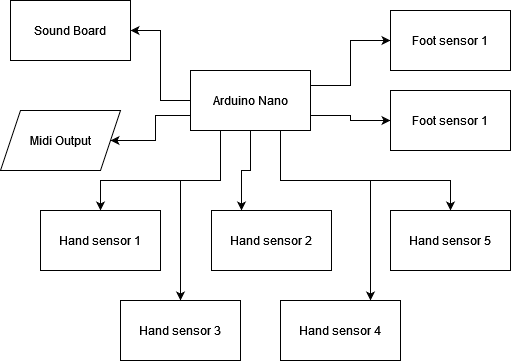
\includegraphics[width=0.75\textwidth]{HW2/BlockDiagram.png}
    \caption{Block diagram of the \textbf{AirDrums}}
    \label{hw1:fig:blockdiagram}
\end{figure}

\section*{Final Project}

This week I researched options for sensors.
\begin{itemize}
    \item  For hand sensors (sensing when the hand strikes the thigh) my main 2 options are Piezo Contact Microphones and Accelerometers.

\item For the right foot sensor I am considering using an accelerometer mounted on the toe of the shoe, I theorize that it should experience a spike in acceleration when the foot strikes the ground.

\item For the left foot sensor I am also considering using an accelerometer. The left foot needs to sense the actual position of the foot since that constrols the sound from the HiHats. 

\end{itemize}
Next week I intend to source some simple accelerometers with analog outputs and some piexo contact microphones and test them out, try to measure the signal to noise ratio.

\end{document}

